
Mechanical, optical and thermal properties at room and cryogenic temperature have been reported in the references \cite{Franc2009,Nawrodt2009_ET}. The following tables and graphs will summarise the different parameters taken into account for thermal noise simulations for the LF and HF interferometers. Generally, at cryogenic temperatures we have listed the values at 10\,K unless otherwise stated.

\FloatBarrier
\subsection{Optics properties data base}\label{app:opticsdb}

The following tables report different optical parameters of bulk and coating materials at room and cryogenic temperature that have been used within this design study.

The bulk materials under investigation for the Einstein Telescope are silicon, sapphire and fused silica. Fused silica is known to be the best currently available optical material at room temperature. For the cryogenic case, silicon and sapphire are the two candidate materials. The detailed discussion of the materials under investigation can be found in Sec.\,\ref{sec:optcomps}.
% % Table 1 : Coating materials _ optic properties _ Room temperature
\begin{table}[h!]
\begin{center}
\begin{tabular}{|l r||r|r|r|}
  \hline
  {\large\strut} Material  & & Fused silica & Silicon & Sapphire \\
  \hline
  \hline
  {\large\strut} Absorption & ppm & 0.25 \cite{BSAbsorbHild2006} & 0.032 @\,1450 nm \cite{Green1995} & 50  \cite{Yan2006} \\
  {\large\strut} Thermo-optic coefficient $\beta$ & (10$^{-6}$/K) & 10 & 13 & - \\
  {\large\strut} Refractive index n & & 1.45 & 3.45 @ 1550\,nm & 1.75\\
 \hline
\end{tabular}
\caption{Optical bulk material properties at room temperature. The refractive index is given at 1064\,nm for fused silica and sapphire.}
\end{center}
\label{tab:Optics_Bulk_Param}
\end{table}

% % Table 2 : Bulk materials _ optic properties _ Cryogenic temperature
\begin{table}[h!]
\begin{center}
\begin{tabular}{|l r||r|r|r|}
  \hline
    {\large\strut} Material  & & Fused silica & Silicon & Sapphire \\
  \hline
  \hline
  {\large\strut} Absorption & ppm & - & - & 90 \cite{Tomaru2001} \\
  {\large\strut} \parbox{0.1\linewidth} {Thermo-optic \\ coefficient$\beta$}  & (10$^{-6}$/K) & 1.01 @ 30\,K & 5.8 @ 30\,K & 0.09 @ 4\,K \\
  {\large\strut} Refractive index n & & 1.44876 @ 30\,K & 3.45 @ 30\,K & 1.75\\
 \hline
\end{tabular}
\caption{Optical bulk material properties at cryogenic temperatures. Parameters are given at 10\,K unless otherwise specified. The refractive index of fused silica and sapphire is given at 1064\,nm whereas for silicon at 1550\,nm.}
\end{center}
\label{tab:Optics_Bulk_Param_cryo}
\end{table}

\FloatBarrier

Several coating materials have been tested as HR coating materials and results have been reported in literature. A report has been devoted to summarize all these parameters values \cite{Franc2009}.

% % Table 3 : Coating materials _ optic properties _ Room temperature
\begin{table}[h!]
\begin{center}
\begin{tabular}{|l r||r|r|r|r|r|r|r|r|}
  \hline
    {\large\strut} Material  & & SiO$_2$ & Al$_2$O$_3$ & Ti:Ta$_2$O$_5$ & Ta$_2$O$_5$ & TiO$_2$ & Nb$_2$O$_5$ & ZrO$_2$ & HfO$_2$ \\
  \hline
  \hline
   {\large\strut} Absorption & ppm & 0.3 \cite{Flaminio2010} & - & 0.5 \cite{Flaminio2010} & 1.22 \cite{Flaminio2010} & - & 2.2 \cite{Flaminio2010} & 11 \cite{Flaminio2010} & - \\
   {\large\strut} \parbox{0.1\linewidth} {Thermo-optic \\ coefficient$\beta$}  & (10$^{-6}$K) &  8 & 13 & 14 & 2.3 & -1.8 & 14.3 & 100 & - \\
   {\large\strut} refractive index n & & 1.45 \cite{Flaminio2010} & 1.58 & 2.06 \cite{Flaminio2010} & 2.035 \cite{Flaminio2010} & 2.11 \cite{Song2008} & 2.21 \cite{Flaminio2010} & 2.1 \cite{Flaminio2010} & 1.985 \cite{Dai2009} \\
  \hline
\end{tabular}
\caption{Optical coating material properties at room temperature -- refractive indices n are given at 1064 nm.}
\end{center}
\label{tab:Optic_Coat_Param}
\end{table}

% % Table 4 : Coating materials _ optic properties _ Cryogenic temperature
\begin{table}[h!]
\begin{center}
\begin{tabular}{|l r||r|r|r|r|r|}
  \hline
    {\large\strut} Material  & & SiO$_2$ & Al$_2$O$_3$ & Ta$_2$O$_5$ & TiO$_2$ & HfO$_2$ \\
  \hline
  \hline
   {\large\strut} Absorption & ppm & - & - & - & - & - \\
   {\large\strut} \parbox{0.1\linewidth} {Thermo-optic \\ coefficient$\beta$}  & (10$^{-6}$K) &  1.01 & - & - & -& -  \\
   {\large\strut} Refractive index @ 1064 nm & & 1.44876 @ 30\,K & - & 2.05 & - & -\\
  \hline
\end{tabular}
\caption{Optical coating material properties at cryogenic temperatures. Parameters are given at 10\,K unless otherwise specified.}
\end{center}
\label{tab:Optic_Coat_Param_cryo}
\end{table}

\FloatBarrier
\subsection{Mechanical properties of optical materials}\label{app:mechdat}
%\emph{Authors: R. Nawrodt, J. Franc, etc.}

The mechanical properties like the Young's modulus, the mass density, Poisson's ratio as well as the mechanical loss angle play an important role in the determination of the Brownian thermal noise contribution. These values are summarised in this section for the bulk and coating materials discussed in this design study -- both at room temperature as well as cryogenic temperatures. Apart from the mechanical loss angle all mechanical properties are only weakly temperature dependent and thus assumed to be temperature independent. The mechanical loss is strongly temperature dependent and thus differently taken into account at different temperatures.

The references for the different values can be found in \cite{Franc2009, Nawrodt2009_ET} unless otherwise stated.

% % Table 5 : Bulk materials _ mechanical properties _ Room temperature
\begin{table}[h!]
\begin{center}
\begin{tabular}{|l r||r|r|r|r|r|}
  \hline
    {\large\strut} Material  & & Fused silica & Si(100) & Si(110) & Si(111) & Sapphire \\
  \hline
  \hline
   {\large\strut} Loss Angle (290\,K) & & $4\times10^{-10}$ & $1\times10^{-8}$ & $1\times10^{-8}$ & $1\times10^{-8}$ & $2\times10^{-9}$ \\
   {\large\strut} Loss Angle (10\,K)  & & $1\times10^{-3} $ & $1\times10^{-9}$ & $1\times10^{-9}$ & $1\times10^{-9}$ & $4\times10^{-9}$ @ 4.2\,K \\
   {\large\strut} Density $\rho$ & (kg/m$^3$) & 2200 & 2330 & 2330 & 2330 & 3980\\
   {\large\strut} Young Modulus E & (GPa) &  72 & 130 & 169 & 188 & 400\\
   {\large\strut} Poisson ratio & & 0.17 & 0.22 & 0.22 & 0.22 & 0.235\\
  \hline
\end{tabular}
\caption{Mechanical bulk material properties at room temperature as well as cryogenic temperatures.}
\end{center}
\label{tab:Mech_Bulk_Param}
\end{table}

% % Table 7 : Low refractive index Coating materials _ mechanical properties _ Room temperature

\begin{table}[h!]
\begin{center}
\begin{tabular}{|l r||r|r|}
  \hline
    {\large\strut} Material  & & SiO$_2$ & Al$_2$O$_3$ \\
  \hline
  \hline
   {\large\strut} Loss Angle & & $0.5\times 10^{-4}$ & $2.4\times 10^{-4}$  \\
   {\large\strut} Density $\rho$ & (kg/m$^3$) & 2200 & 3700 \\
   {\large\strut} Young Modulus E & (GPa) &  60 & 210\\
   {\large\strut} Poisson ratio & & 0.17 & 0.22 \\
  \hline
\end{tabular}
\caption{Low refractive index materials -- Mechanical properties at room temperature.}
\end{center}
\label{tab:Mech_CoatLowRef_Param}
\end{table}

% % Table 8 : High refractive index Coating materials _ mechanical properties _ Room temperature
\begin{table}[h!]
\begin{center}
\begin{tabular}{|l r||r|r|r|r|r|r|}
  \hline
    {\large\strut} Material  & & Ti:Ta$_2$O$_5$ & Ta$_2$O$_5$ & TiO$_2$ & Nb$_2$O$_5$ & ZrO$_2$ & HfO$_2$ \\
  \hline
  \hline
   {\large\strut} Loss Angle & &  $2\times 10^{-4}$ & $3.8\times 10^{-4}$  & $6.3\times 10^{-3}$ & $4.6\times 10^{-4}$ & $2.3\times 10^{-4}$ & $5.9\times 10^{-4}$  \\
   {\large\strut} Density $\rho$ & (kg/m$^3$) & 6425 & 6850 & 4230 & 4590 & 6000 & 8000 \\
   {\large\strut} Young Modulus E & (GPa) & 140 & 140 & 290 & 68 & 200 & 380 \\
   {\large\strut} Poisson ratio & & 0.23 & 0.23 & 0.28 & 0.2 & 0.27 & 0.2 \\
  \hline
\end{tabular}
\caption{High refractive index materials -- Mechanical properties at room temperature.}
\end{center}
\label{tab:Mech_CoatHighRef_Param}
\end{table}

% % Table 9 : Coating materials _ mechanical properties _ Cryogenic temperature
\begin{table}[h!]
\begin{center}
\begin{tabular}{|l r||r|r|r|r|r|}
  \hline
    {\large\strut} Material  & & SiO$_2$ & Al$_2$O$_3$ &  Ti:Ta$_2$O$_5$ & TiO$_2$ & HfO$_2$ \\
  \hline
  \hline
   {\large\strut} Loss Angle & & $5\times10^{-4}$ & - & $3.8\times 10^{-4}$ & $5.6\times 10^{-3}$ @ 77\,K & $2.2\times 10^{-4}$  \\
   {\large\strut} Density $\rho$ & (kg/m$^3$) & 2200 & 3700 & 6425 & 4269 @ 73\,K & - \\
   {\large\strut} Young Modulus E & (GPa) &  60 & 356 & 140 & 290 & - \\
   {\large\strut} Poisson ratio & & 0.159 & 0.2 & 0.21 & 0.253 & - \\
  \hline
\end{tabular}
\caption{Mechanical coating material properties at cryogenic temperatures. Parameters are given at 10\,K unless otherwise specified.}
\end{center}
\label{tab:Mech_Coat_Param_cryo}
\end{table}


\FloatBarrier
\subsection{Thermal properties of optical materials}
\label{app:thermdat}
%\emph{Authors: R. Nawrodt, J. Franc, etc.}

This section summarises the thermal properties of bulk and coating materials at room and cryogenic temperatures. These parameters influence the thermo-elastic and thermo-refractive noise contributions from the different components.

The references for the different values can be found in \cite{Franc2009, Nawrodt2009_ET} unless otherwise stated.

% % Table 10 : Bulk materials _ Thermal properties _ Room temperature
\begin{table}[h!]
\begin{center}
\begin{tabular}{|l r||r|r|r|}
  \hline
    {\large\strut} Material  & & Fused silica & Silicon & Sapphire \\
  \hline
  \hline
   {\large\strut} Thermal conductivity k$_{th}$ & (W/m K) & 1.38  & 130-160  & 33 \\
   {\large\strut} Specific heat C & (J/kg K) & 746  & 711  & 770\\
   {\large\strut} Thermal expansion $\alpha$ & ($10^{-6}$/K) &  0.51  & 2.54 & 5.1\\
     \hline
\end{tabular}
\end{center}
\caption{Thermal bulk material properties at room temperature.}
\label{tab:Therm_Bulk_Param_room}
\end{table}

% % Table 11 : Bulk materials _ Thermal properties _ Cryogenic temperature
\begin{table}[h!]
\begin{center}
\begin{tabular}{|l r||r|r|r|}
  \hline
    {\large\strut} Material  & & Fused silica & Silicon & Sapphire \\
  \hline
  \hline
   {\large\strut} Thermal conductivity k$_{th}$ & (W/m K) & 0.4 & 2330 & 1500 @ 12.5\,K \\
   {\large\strut} Specific heat C & (J/kg K) & 3 & 0.276 & $9.34\times 10^{-2}$ @ 10\,K \\
   {\large\strut} Thermal expansion $\alpha$ & (1/K) &  $ -0.25\times 10^{-6}$ & $4.85\times10^{-10}$ & $5.3\times10^{-10}$ \\
  \hline
\end{tabular}
\caption{Thermal bulk material properties at cryogenic temperatures. }
\end{center}
\label{tab:Therm_Bulk_Param_cryo}
\end{table}

\begin{figure}[h!]
\begin{center}
\subfigure[]{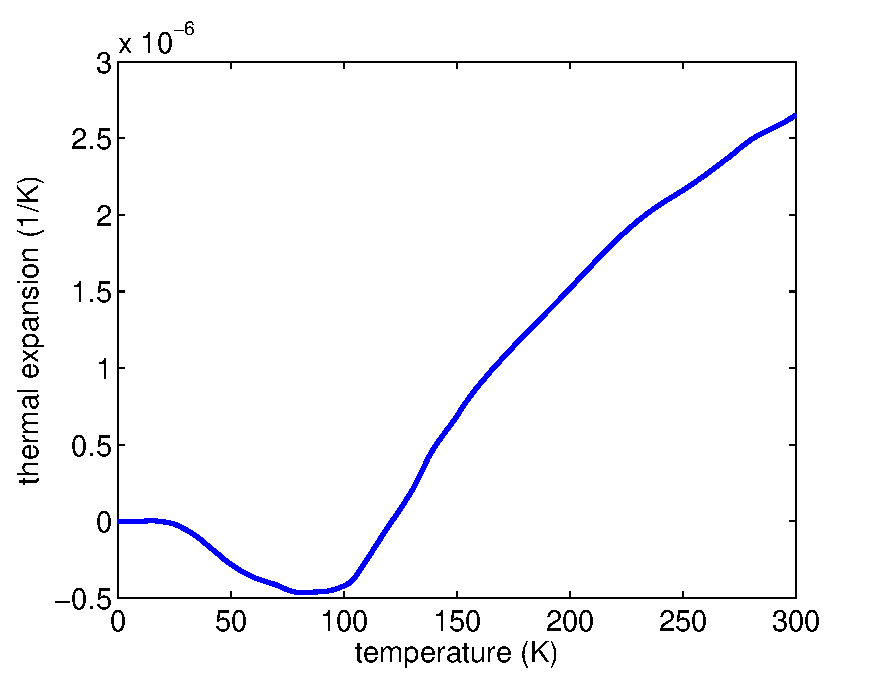
\includegraphics[width=0.4\linewidth]{Appendices/Figures/Si_alpha.pdf}}
\subfigure[]{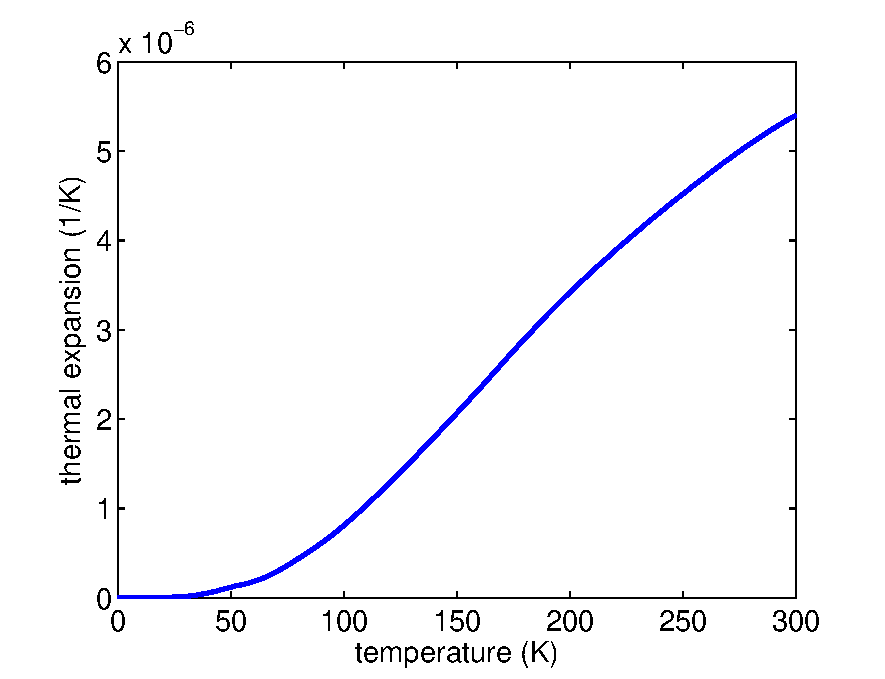
\includegraphics[width=0.4\linewidth]{Appendices/Figures/Sapphire_alpha.pdf}}
\caption{Dependence of the coefficient of thermal expansion for silicon (a) and sapphire (b) as a function of temperature.}
\end{center}
\label{fig:app_alpha}
\end{figure}

\begin{figure}[h!]
\begin{center}
\subfigure[]{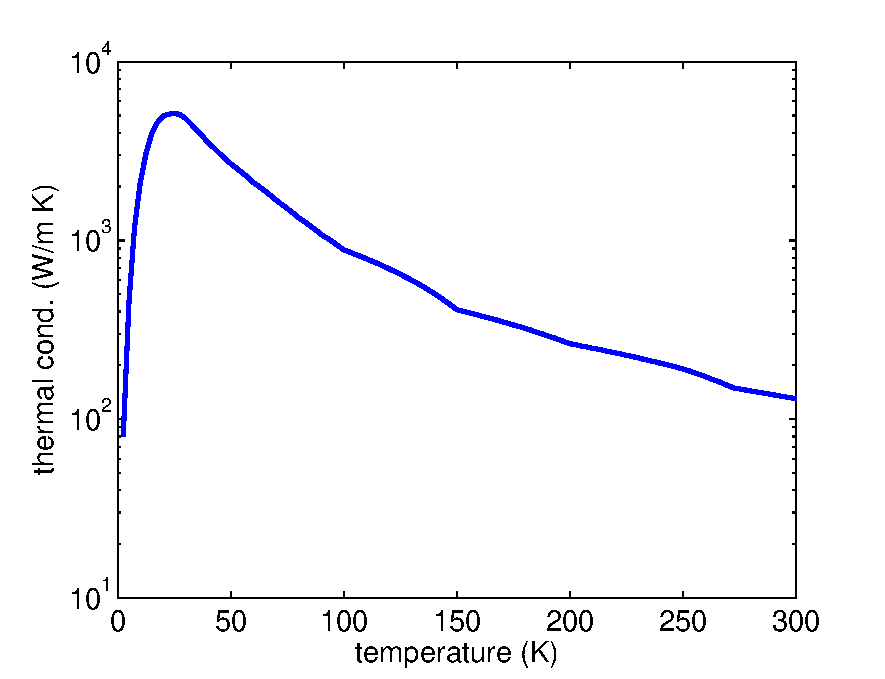
\includegraphics[width=0.4\linewidth]{Appendices/Figures/Si_kappa.pdf}}
\subfigure[]{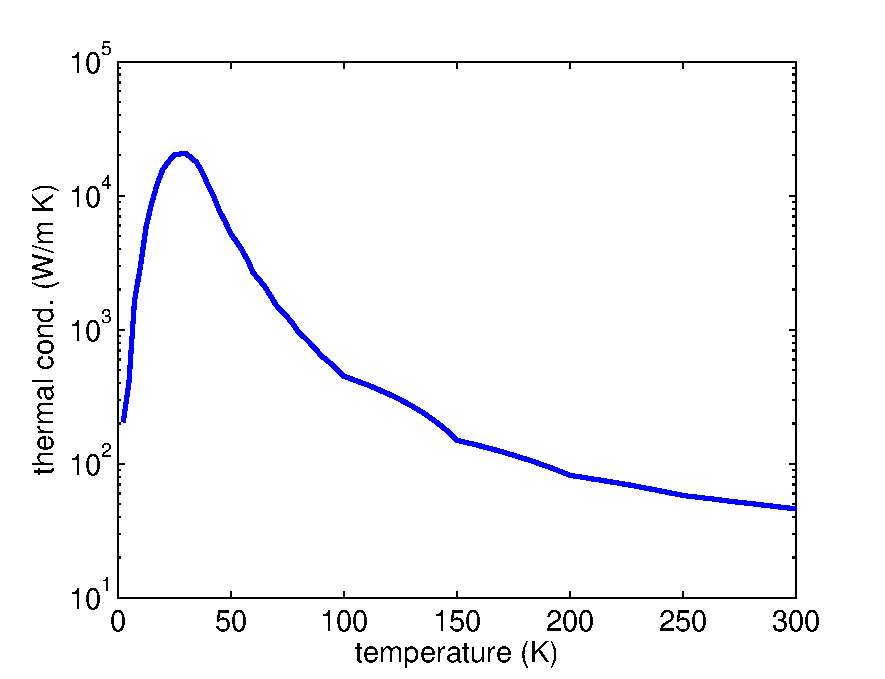
\includegraphics[width=0.4\linewidth]{Appendices/Figures/Sapphire_kappa.pdf}}
\caption{Dependence of the thermal conductivity of silicon (a) and sapphire (b) as a function of temperature.}
\end{center}
\label{fig:app_kappa}
\end{figure}

\begin{figure}[h!]
\begin{center}
\subfigure[]{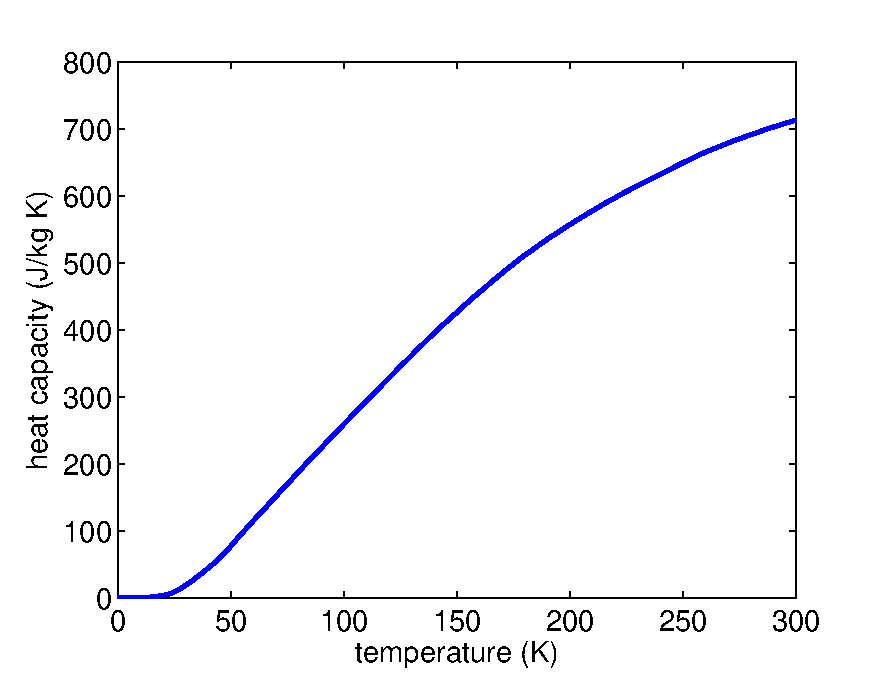
\includegraphics[width=0.4\linewidth]{Appendices/Figures/Si_Cp.pdf}}
\subfigure[]{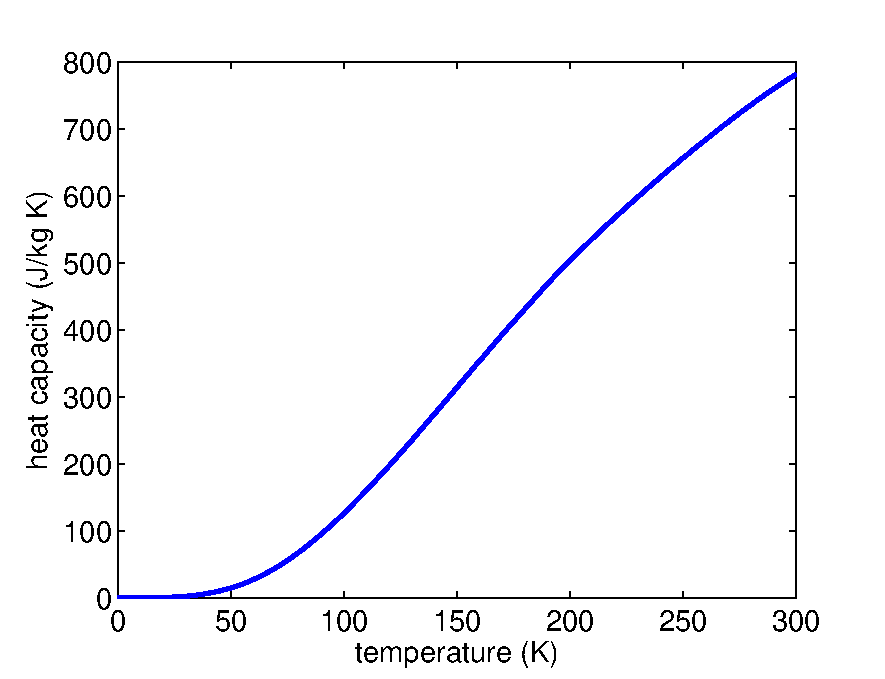
\includegraphics[width=0.4\linewidth]{Appendices/Figures/Sapphire_Cp.pdf}}
\caption{Dependence of the heat capacity of silicon (a) and sapphire (b) as a function of temperature.}
\end{center}
\label{fig:app_Cp}
\end{figure}

% % Table 12 : Low refractive index Coating materials _ Thermal properties _ Room temperature
\begin{table}[h!]
\begin{center}
\begin{tabular}{|l r||r|r|}
  \hline
    {\large\strut} Material  & & SiO$_2$ & Al$_2$O$_3$ \\
  \hline
  \hline
   {\large\strut} Thermal conductivity k$_{th}$ & (W/m K) & 0.5  & 3.3 \\
   {\large\strut} Specific heat C & (J/kg K) & 746  & 310 \\
   {\large\strut} Thermal expansion $\alpha$ & ($10^{-6}$/K) &  0.51  & 8.4 \\
    \hline
\end{tabular}
\caption{Thermal properties of low refractive index materials at room temperature.}
\end{center}
\label{tab:Therm_CoatLowRef_Param}
\end{table}

% Table 13 : High refractive Coating materials _ Thermal properties _ Room temperature
\begin{table}[h!]
\begin{center}
\begin{tabular}{|l r||r|r|r|r|r|r|}
  \hline 
   {\large\strut} Material  & & Ti:Ta$_2$O$_5$ & Ta$_2$O$_5$ & TiO$_2$ & Nb$_2$O$_5$ & ZrO$_2$ & HfO$_2$ \\ \hline \hline
   {\large\strut} Thermal conductivity k$_{th}$ & (W/m K) & 0.6 & 0.6 & 0.45 & 1 & 1.09 & 1.2 \\
   {\large\strut} Specific heat C & (J/kg K) & 269 & 306 & 130 & 590 & 26 & 16.7 \\
   {\large\strut} Thermal expansion $\alpha$ & ($10^{-6}$/K) & 3.6 & 3.6 & 50 & 5.8 & 10.3 & 3.8 \\
  \hline
\end{tabular}
\caption{Thermal properties of high refractive index materials at room temperature.}
\end{center}
\label{tab:Therm_CoatHighRef_Param}
\end{table}

% % Table 14 : Coating materials _ Thermal properties _ Cryogenic temperature
\begin{table}[h!]
\begin{center}
\begin{tabular}{|l r||r|r|r|r|r|}
  \hline
    {\large\strut} Material  & & SiO$_2$ & Al$_2$O$_3$ & Ti:Ta$_2$O$_5$ & TiO$_2$ & HfO$_2$ \\
  \hline
  \hline
   {\large\strut} Thermal conductivity k$_{th}$ & (W/m K) & 0.13  & 5 & - & 500 & - \\
   {\large\strut} Specific heat C & (J/kg K) & 1-7  &  0.1 & 3.17 @ 50\,K & 0.012 & - \\
   {\large\strut} Thermal expansion $\alpha$ & ($10^{-6}$/K) & -0.25 & 0.6 @ 100\,K & - & 6.5 @ 100\,K & - \\
     \hline
\end{tabular}
\caption{Thermal coating material properties at cryogenic temperatures. All parameters are given at 10\,K unless otherwise stated.}
\end{center}
\label{tab:Therm_Coat_Param_cryo}
\end{table}

